% Requires: \usepackage{tikz}  \usetikzlibrary{calc}
% Place inside \begin{figure}...\end{figure} with \resizebox{\textwidth}{!}{...}
\definecolor{ftT}{HTML}{E3EDFA}\definecolor{ftTb}{HTML}{2A78D6}
\definecolor{ftH}{HTML}{FDEBD9}\definecolor{ftHb}{HTML}{C26A14}
\definecolor{ftO}{HTML}{EFE6F6}\definecolor{ftOb}{HTML}{7C3AED}
\definecolor{ftE}{HTML}{E6F2E0}\definecolor{ftEb}{HTML}{3F7D2A}
\definecolor{ftG}{HTML}{1F2937}\definecolor{ftL}{HTML}{6B7280}\definecolor{ftR}{HTML}{B91C1C}
\newcommand{\ftor}[2]{\draw[ftG,fill=white,line width=0.4pt] (#1,#2+0.15) .. controls (#1+0.25,#2+0.15) and (#1+0.43,#2+0.075) .. (#1+0.5,#2) .. controls (#1+0.43,#2-0.075) and (#1+0.25,#2-0.15) .. (#1,#2-0.15) .. controls (#1+0.12,#2-0.075) and (#1+0.12,#2+0.075) .. (#1,#2+0.15); \node[font=\fontsize{4.2}{4.6}\selectfont\bfseries,ftG] at (#1+0.23,#2) {OR};}
\newcommand{\ftand}[2]{\draw[ftG,fill=ftG,line width=0.4pt] (#1,#2+0.15) -- (#1+0.23,#2+0.15) .. controls (#1+0.43,#2+0.15) and (#1+0.5,#2+0.075) .. (#1+0.5,#2) .. controls (#1+0.5,#2-0.075) and (#1+0.43,#2-0.15) .. (#1+0.23,#2-0.15) -- (#1,#2-0.15) -- cycle; \node[font=\fontsize{3.2}{3.6}\selectfont\bfseries,white] at (#1+0.22,#2) {AND};}
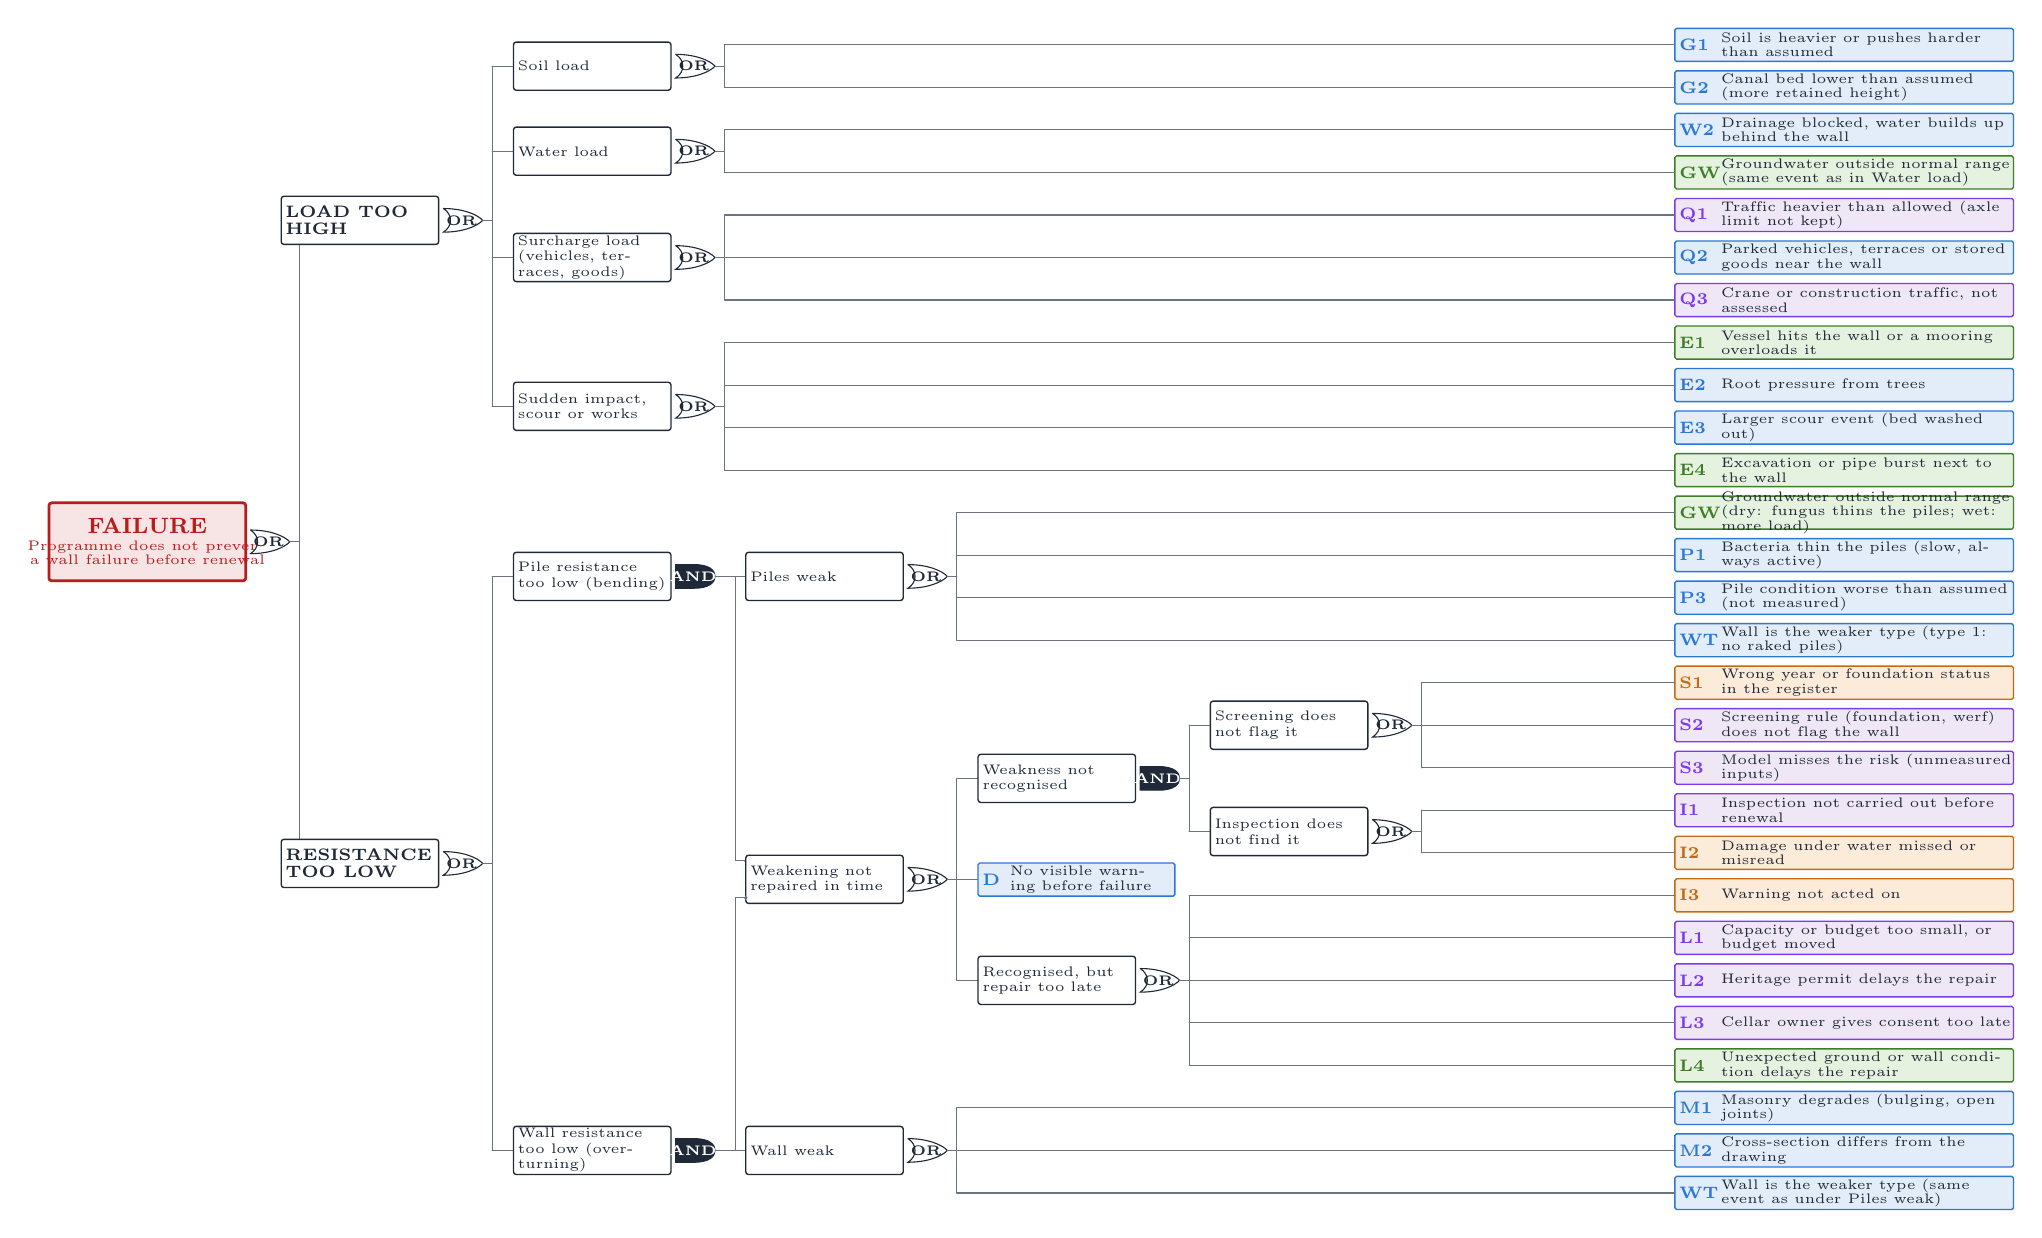
\begin{tikzpicture}[x=1cm,y=1cm,line cap=round,every node/.style={inner sep=0pt}]
\tikzset{ftline/.style={ftL,line width=0.4pt}}

\draw[ftTb,fill=ftT,line width=0.5pt,rounded corners=0.6pt] (20.75,-6.69) rectangle (25.05,-6.27);
\node[anchor=west,font=\fontsize{6}{6}\selectfont\bfseries,ftTb] at (20.8,-6.48) {P1};
\node[anchor=west,text width=3.7cm,font=\fontsize{4.8}{5.2}\selectfont,ftG] at (21.33,-6.48) {Bacteria thin the piles (slow, always active)};
\draw[ftTb,fill=ftT,line width=0.5pt,rounded corners=0.6pt] (20.75,-7.23) rectangle (25.05,-6.81);
\node[anchor=west,font=\fontsize{6}{6}\selectfont\bfseries,ftTb] at (20.8,-7.02) {P3};
\node[anchor=west,text width=3.7cm,font=\fontsize{4.8}{5.2}\selectfont,ftG] at (21.33,-7.02) {Pile condition worse than assumed (not measured)};
\draw[ftTb,fill=ftT,line width=0.5pt,rounded corners=0.6pt] (20.75,-13.71) rectangle (25.05,-13.29);
\node[anchor=west,font=\fontsize{6}{6}\selectfont\bfseries,ftTb] at (20.8,-13.5) {M1};
\node[anchor=west,text width=3.7cm,font=\fontsize{4.8}{5.2}\selectfont,ftG] at (21.33,-13.5) {Masonry degrades (bulging, open joints)};
\draw[ftTb,fill=ftT,line width=0.5pt,rounded corners=0.6pt] (20.75,-14.25) rectangle (25.05,-13.83);
\node[anchor=west,font=\fontsize{6}{6}\selectfont\bfseries,ftTb] at (20.8,-14.04) {M2};
\node[anchor=west,text width=3.7cm,font=\fontsize{4.8}{5.2}\selectfont,ftG] at (21.33,-14.04) {Cross-section differs from the drawing};
\draw[ftTb,fill=ftT,line width=0.5pt,rounded corners=0.6pt] (20.75,-7.77) rectangle (25.05,-7.35);
\node[anchor=west,font=\fontsize{6}{6}\selectfont\bfseries,ftTb] at (20.8,-7.56) {WT};
\node[anchor=west,text width=3.7cm,font=\fontsize{4.8}{5.2}\selectfont,ftG] at (21.33,-7.56) {Wall is the weaker type (type 1: no raked piles)};
\draw[ftEb,fill=ftE,line width=0.5pt,rounded corners=0.6pt] (20.75,-1.83) rectangle (25.05,-1.41);
\node[anchor=west,font=\fontsize{6}{6}\selectfont\bfseries,ftEb] at (20.8,-1.62) {GW};
\node[anchor=west,text width=3.7cm,font=\fontsize{4.8}{5.2}\selectfont,ftG] at (21.33,-1.62) {Groundwater outside normal range (same event as in Water load)};
\draw[ftTb,fill=ftT,line width=0.5pt,rounded corners=0.6pt] (20.75,-14.79) rectangle (25.05,-14.37);
\node[anchor=west,font=\fontsize{6}{6}\selectfont\bfseries,ftTb] at (20.8,-14.58) {WT};
\node[anchor=west,text width=3.7cm,font=\fontsize{4.8}{5.2}\selectfont,ftG] at (21.33,-14.58) {Wall is the weaker type (same event as under Piles weak)};
\draw[ftEb,fill=ftE,line width=0.5pt,rounded corners=0.6pt] (20.75,-6.15) rectangle (25.05,-5.73);
\node[anchor=west,font=\fontsize{6}{6}\selectfont\bfseries,ftEb] at (20.8,-5.94) {GW};
\node[anchor=west,text width=3.7cm,font=\fontsize{4.8}{5.2}\selectfont,ftG] at (21.33,-5.94) {Groundwater outside normal range (dry: fungus thins the piles; wet: more load)};
\draw[ftTb,fill=ftT,line width=0.5pt,rounded corners=0.6pt] (20.75,-0.21) rectangle (25.05,0.21);
\node[anchor=west,font=\fontsize{6}{6}\selectfont\bfseries,ftTb] at (20.8,-0.0) {G1};
\node[anchor=west,text width=3.7cm,font=\fontsize{4.8}{5.2}\selectfont,ftG] at (21.33,-0.0) {Soil is heavier or pushes harder than assumed};
\draw[ftTb,fill=ftT,line width=0.5pt,rounded corners=0.6pt] (20.75,-0.75) rectangle (25.05,-0.33);
\node[anchor=west,font=\fontsize{6}{6}\selectfont\bfseries,ftTb] at (20.8,-0.54) {G2};
\node[anchor=west,text width=3.7cm,font=\fontsize{4.8}{5.2}\selectfont,ftG] at (21.33,-0.54) {Canal bed lower than assumed (more retained height)};
\draw[ftTb,fill=ftT,line width=0.5pt,rounded corners=0.6pt] (20.75,-1.29) rectangle (25.05,-0.87);
\node[anchor=west,font=\fontsize{6}{6}\selectfont\bfseries,ftTb] at (20.8,-1.08) {W2};
\node[anchor=west,text width=3.7cm,font=\fontsize{4.8}{5.2}\selectfont,ftG] at (21.33,-1.08) {Drainage blocked, water builds up behind the wall};
\draw[ftOb,fill=ftO,line width=0.5pt,rounded corners=0.6pt] (20.75,-2.37) rectangle (25.05,-1.95);
\node[anchor=west,font=\fontsize{6}{6}\selectfont\bfseries,ftOb] at (20.8,-2.16) {Q1};
\node[anchor=west,text width=3.7cm,font=\fontsize{4.8}{5.2}\selectfont,ftG] at (21.33,-2.16) {Traffic heavier than allowed (axle limit not kept)};
\draw[ftTb,fill=ftT,line width=0.5pt,rounded corners=0.6pt] (20.75,-2.91) rectangle (25.05,-2.49);
\node[anchor=west,font=\fontsize{6}{6}\selectfont\bfseries,ftTb] at (20.8,-2.7) {Q2};
\node[anchor=west,text width=3.7cm,font=\fontsize{4.8}{5.2}\selectfont,ftG] at (21.33,-2.7) {Parked vehicles, terraces or stored goods near the wall};
\draw[ftOb,fill=ftO,line width=0.5pt,rounded corners=0.6pt] (20.75,-3.45) rectangle (25.05,-3.03);
\node[anchor=west,font=\fontsize{6}{6}\selectfont\bfseries,ftOb] at (20.8,-3.24) {Q3};
\node[anchor=west,text width=3.7cm,font=\fontsize{4.8}{5.2}\selectfont,ftG] at (21.33,-3.24) {Crane or construction traffic, not assessed};
\draw[ftEb,fill=ftE,line width=0.5pt,rounded corners=0.6pt] (20.75,-3.99) rectangle (25.05,-3.57);
\node[anchor=west,font=\fontsize{6}{6}\selectfont\bfseries,ftEb] at (20.8,-3.78) {E1};
\node[anchor=west,text width=3.7cm,font=\fontsize{4.8}{5.2}\selectfont,ftG] at (21.33,-3.78) {Vessel hits the wall or a mooring overloads it};
\draw[ftTb,fill=ftT,line width=0.5pt,rounded corners=0.6pt] (20.75,-4.53) rectangle (25.05,-4.11);
\node[anchor=west,font=\fontsize{6}{6}\selectfont\bfseries,ftTb] at (20.8,-4.32) {E2};
\node[anchor=west,text width=3.7cm,font=\fontsize{4.8}{5.2}\selectfont,ftG] at (21.33,-4.32) {Root pressure from trees};
\draw[ftTb,fill=ftT,line width=0.5pt,rounded corners=0.6pt] (20.75,-5.07) rectangle (25.05,-4.65);
\node[anchor=west,font=\fontsize{6}{6}\selectfont\bfseries,ftTb] at (20.8,-4.86) {E3};
\node[anchor=west,text width=3.7cm,font=\fontsize{4.8}{5.2}\selectfont,ftG] at (21.33,-4.86) {Larger scour event (bed washed out)};
\draw[ftEb,fill=ftE,line width=0.5pt,rounded corners=0.6pt] (20.75,-5.61) rectangle (25.05,-5.19);
\node[anchor=west,font=\fontsize{6}{6}\selectfont\bfseries,ftEb] at (20.8,-5.4) {E4};
\node[anchor=west,text width=3.7cm,font=\fontsize{4.8}{5.2}\selectfont,ftG] at (21.33,-5.4) {Excavation or pipe burst next to the wall};
\draw[ftHb,fill=ftH,line width=0.5pt,rounded corners=0.6pt] (20.75,-8.31) rectangle (25.05,-7.89);
\node[anchor=west,font=\fontsize{6}{6}\selectfont\bfseries,ftHb] at (20.8,-8.1) {S1};
\node[anchor=west,text width=3.7cm,font=\fontsize{4.8}{5.2}\selectfont,ftG] at (21.33,-8.1) {Wrong year or foundation status in the register};
\draw[ftOb,fill=ftO,line width=0.5pt,rounded corners=0.6pt] (20.75,-8.85) rectangle (25.05,-8.43);
\node[anchor=west,font=\fontsize{6}{6}\selectfont\bfseries,ftOb] at (20.8,-8.64) {S2};
\node[anchor=west,text width=3.7cm,font=\fontsize{4.8}{5.2}\selectfont,ftG] at (21.33,-8.64) {Screening rule (foundation, werf) does not flag the wall};
\draw[ftOb,fill=ftO,line width=0.5pt,rounded corners=0.6pt] (20.75,-9.39) rectangle (25.05,-8.97);
\node[anchor=west,font=\fontsize{6}{6}\selectfont\bfseries,ftOb] at (20.8,-9.18) {S3};
\node[anchor=west,text width=3.7cm,font=\fontsize{4.8}{5.2}\selectfont,ftG] at (21.33,-9.18) {Model misses the risk (unmeasured inputs)};
\draw[ftOb,fill=ftO,line width=0.5pt,rounded corners=0.6pt] (20.75,-9.93) rectangle (25.05,-9.51);
\node[anchor=west,font=\fontsize{6}{6}\selectfont\bfseries,ftOb] at (20.8,-9.72) {I1};
\node[anchor=west,text width=3.7cm,font=\fontsize{4.8}{5.2}\selectfont,ftG] at (21.33,-9.72) {Inspection not carried out before renewal};
\draw[ftHb,fill=ftH,line width=0.5pt,rounded corners=0.6pt] (20.75,-10.47) rectangle (25.05,-10.05);
\node[anchor=west,font=\fontsize{6}{6}\selectfont\bfseries,ftHb] at (20.8,-10.26) {I2};
\node[anchor=west,text width=3.7cm,font=\fontsize{4.8}{5.2}\selectfont,ftG] at (21.33,-10.26) {Damage under water missed or misread};
\draw[ftHb,fill=ftH,line width=0.5pt,rounded corners=0.6pt] (20.75,-11.01) rectangle (25.05,-10.59);
\node[anchor=west,font=\fontsize{6}{6}\selectfont\bfseries,ftHb] at (20.8,-10.8) {I3};
\node[anchor=west,text width=3.7cm,font=\fontsize{4.8}{5.2}\selectfont,ftG] at (21.33,-10.8) {Warning not acted on};
\draw[ftOb,fill=ftO,line width=0.5pt,rounded corners=0.6pt] (20.75,-11.55) rectangle (25.05,-11.13);
\node[anchor=west,font=\fontsize{6}{6}\selectfont\bfseries,ftOb] at (20.8,-11.34) {L1};
\node[anchor=west,text width=3.7cm,font=\fontsize{4.8}{5.2}\selectfont,ftG] at (21.33,-11.34) {Capacity or budget too small, or budget moved};
\draw[ftOb,fill=ftO,line width=0.5pt,rounded corners=0.6pt] (20.75,-12.09) rectangle (25.05,-11.67);
\node[anchor=west,font=\fontsize{6}{6}\selectfont\bfseries,ftOb] at (20.8,-11.88) {L2};
\node[anchor=west,text width=3.7cm,font=\fontsize{4.8}{5.2}\selectfont,ftG] at (21.33,-11.88) {Heritage permit delays the repair};
\draw[ftOb,fill=ftO,line width=0.5pt,rounded corners=0.6pt] (20.75,-12.63) rectangle (25.05,-12.21);
\node[anchor=west,font=\fontsize{6}{6}\selectfont\bfseries,ftOb] at (20.8,-12.42) {L3};
\node[anchor=west,text width=3.7cm,font=\fontsize{4.8}{5.2}\selectfont,ftG] at (21.33,-12.42) {Cellar owner gives consent too late};
\draw[ftEb,fill=ftE,line width=0.5pt,rounded corners=0.6pt] (20.75,-13.17) rectangle (25.05,-12.75);
\node[anchor=west,font=\fontsize{6}{6}\selectfont\bfseries,ftEb] at (20.8,-12.96) {L4};
\node[anchor=west,text width=3.7cm,font=\fontsize{4.8}{5.2}\selectfont,ftG] at (21.33,-12.96) {Unexpected ground or wall condition delays the repair};
\draw[ftR,fill=ftR!12, line width=1pt,rounded corners=1pt] (0.1,-6.806) rectangle (2.6,-5.816);
\node[text=ftR,align=center,font=\fontsize{8.5}{9}\selectfont\bfseries] at (1.35,-6.111) {FAILURE};
\node[text=ftR,align=center,font=\fontsize{4.6}{5.2}\selectfont] at (1.35,-6.451) {Programme does not prevent\\a wall failure before renewal};
\ftor{2.66}{-6.311}
\draw[ftline] (3.16,-6.311) -- (3.28,-6.311);
\draw[ftline] (3.28,-10.395) -- (3.28,-2.228);
\draw[ftline] (3.28,-2.228) -- (3.05,-2.228);
\draw[ftline] (3.28,-10.395) -- (3.05,-10.395);
\draw[ftG,fill=white, line width=0.5pt,rounded corners=1pt] (3.05,-10.701) rectangle (5.05,-10.089);
\node[anchor=west,text width=1.9cm,font=\fontsize{5.6}{6}\selectfont\bfseries,ftG] at (3.1,-10.395) {RESISTANCE TOO LOW};
\ftor{5.11}{-10.395}
\draw[ftline] (5.61,-10.395) -- (5.73,-10.395);
\draw[ftline] (5.73,-14.04) -- (5.73,-6.75);
\draw[ftline] (5.73,-6.75) -- (6.0,-6.75);
\draw[ftline] (5.73,-14.04) -- (6.0,-14.04);
\draw[ftG,fill=white, line width=0.5pt,rounded corners=1pt] (6.0,-7.056) rectangle (8.0,-6.444);
\node[anchor=west,text width=1.9cm,font=\fontsize{5}{5.6}\selectfont,ftG] at (6.05,-6.75) {Pile resistance too low (bending)};
\ftand{8.06}{-6.75}
\draw[ftline] (8.56,-6.75) -- (8.68,-6.75);
\draw[ftline] (8.68,-6.75) -- (8.68,-6.75);
\draw[ftline] (8.68,-6.75) -- (8.95,-6.75);
\draw[ftline] (8.68,-6.75) -- (8.815,-6.75) -- (8.815,-10.361) -- (8.95,-10.361);
\fill[ftL] (8.95,-10.361) circle (0.025);
\draw[ftG,fill=white, line width=0.5pt,rounded corners=1pt] (8.95,-7.056) rectangle (10.95,-6.444);
\node[anchor=west,text width=1.9cm,font=\fontsize{5}{5.6}\selectfont,ftG] at (9.0,-6.75) {Piles weak};
\ftor{11.01}{-6.75}
\draw[ftline] (11.51,-6.75) -- (11.63,-6.75);
\draw[ftline] (11.63,-7.56) -- (11.63,-5.94);
\draw[ftline] (11.63,-5.94) -- (20.75,-5.94);
\draw[ftline] (11.63,-6.48) -- (20.75,-6.48);
\draw[ftline] (11.63,-7.02) -- (20.75,-7.02);
\draw[ftline] (11.63,-7.56) -- (20.75,-7.56);
\draw[ftG,fill=white, line width=0.5pt,rounded corners=1pt] (8.95,-10.903) rectangle (10.95,-10.291);
\node[anchor=west,text width=1.9cm,font=\fontsize{5}{5.6}\selectfont,ftG] at (9.0,-10.597) {Weakening not repaired in time};
\ftor{11.01}{-10.597}
\draw[ftline] (11.51,-10.597) -- (11.63,-10.597);
\draw[ftline] (11.63,-11.88) -- (11.63,-9.315);
\draw[ftline] (11.63,-9.315) -- (11.9,-9.315);
\draw[ftline] (11.63,-11.88) -- (11.9,-11.88);
\draw[ftG,fill=white, line width=0.5pt,rounded corners=1pt] (11.9,-9.621) rectangle (13.9,-9.009);
\node[anchor=west,text width=1.9cm,font=\fontsize{5}{5.6}\selectfont,ftG] at (11.95,-9.315) {Weakness not recognised};
\ftand{13.96}{-9.315}
\draw[ftline] (14.46,-9.315) -- (14.58,-9.315);
\draw[ftline] (14.58,-9.99) -- (14.58,-8.64);
\draw[ftline] (14.58,-8.64) -- (14.85,-8.64);
\draw[ftline] (14.58,-9.99) -- (14.85,-9.99);
\draw[ftG,fill=white, line width=0.5pt,rounded corners=1pt] (14.85,-8.946) rectangle (16.85,-8.334);
\node[anchor=west,text width=1.9cm,font=\fontsize{5}{5.6}\selectfont,ftG] at (14.9,-8.64) {Screening does not flag it};
\ftor{16.91}{-8.64}
\draw[ftline] (17.41,-8.64) -- (17.53,-8.64);
\draw[ftline] (17.53,-9.18) -- (17.53,-8.1);
\draw[ftline] (17.53,-8.1) -- (20.75,-8.1);
\draw[ftline] (17.53,-8.64) -- (20.75,-8.64);
\draw[ftline] (17.53,-9.18) -- (20.75,-9.18);
\draw[ftG,fill=white, line width=0.5pt,rounded corners=1pt] (14.85,-10.296) rectangle (16.85,-9.684);
\node[anchor=west,text width=1.9cm,font=\fontsize{5}{5.6}\selectfont,ftG] at (14.9,-9.99) {Inspection does not find it};
\ftor{16.91}{-9.99}
\draw[ftline] (17.41,-9.99) -- (17.53,-9.99);
\draw[ftline] (17.53,-10.26) -- (17.53,-9.72);
\draw[ftline] (17.53,-9.72) -- (20.75,-9.72);
\draw[ftline] (17.53,-10.26) -- (20.75,-10.26);
\draw[ftline] (11.63,-10.6) -- (11.9,-10.6);
\draw[ftTb,fill=ftT,line width=0.5pt,rounded corners=0.6pt] (11.9,-10.81) rectangle (14.4,-10.39);
\node[anchor=west,font=\fontsize{6}{6}\selectfont\bfseries,ftTb] at (11.95,-10.6) {D};
\node[anchor=west,text width=1.95cm,font=\fontsize{4.8}{5.2}\selectfont,ftG] at (12.3,-10.6) {No visible warning before failure};
\draw[ftG,fill=white, line width=0.5pt,rounded corners=1pt] (11.9,-12.186) rectangle (13.9,-11.574);
\node[anchor=west,text width=1.9cm,font=\fontsize{5}{5.6}\selectfont,ftG] at (11.95,-11.88) {Recognised, but repair too late};
\ftor{13.96}{-11.88}
\draw[ftline] (14.46,-11.88) -- (14.58,-11.88);
\draw[ftline] (14.58,-12.96) -- (14.58,-10.8);
\draw[ftline] (14.58,-10.8) -- (20.75,-10.8);
\draw[ftline] (14.58,-11.34) -- (20.75,-11.34);
\draw[ftline] (14.58,-11.88) -- (20.75,-11.88);
\draw[ftline] (14.58,-12.42) -- (20.75,-12.42);
\draw[ftline] (14.58,-12.96) -- (20.75,-12.96);
\draw[ftG,fill=white, line width=0.5pt,rounded corners=1pt] (6.0,-14.346) rectangle (8.0,-13.734);
\node[anchor=west,text width=1.9cm,font=\fontsize{5}{5.6}\selectfont,ftG] at (6.05,-14.04) {Wall resistance too low (overturning)};
\ftand{8.06}{-14.04}
\draw[ftline] (8.56,-14.04) -- (8.68,-14.04);
\draw[ftline] (8.68,-14.04) -- (8.68,-14.04);
\draw[ftline] (8.68,-14.04) -- (8.95,-14.04);
\draw[ftline] (8.68,-14.04) -- (8.815,-14.04) -- (8.815,-10.833) -- (8.95,-10.833);
\fill[ftL] (8.95,-10.833) circle (0.025);
\draw[ftG,fill=white, line width=0.5pt,rounded corners=1pt] (8.95,-14.346) rectangle (10.95,-13.734);
\node[anchor=west,text width=1.9cm,font=\fontsize{5}{5.6}\selectfont,ftG] at (9.0,-14.04) {Wall weak};
\ftor{11.01}{-14.04}
\draw[ftline] (11.51,-14.04) -- (11.63,-14.04);
\draw[ftline] (11.63,-14.58) -- (11.63,-13.5);
\draw[ftline] (11.63,-13.5) -- (20.75,-13.5);
\draw[ftline] (11.63,-14.04) -- (20.75,-14.04);
\draw[ftline] (11.63,-14.58) -- (20.75,-14.58);
\draw[ftG,fill=white, line width=0.5pt,rounded corners=1pt] (3.05,-2.534) rectangle (5.05,-1.922);
\node[anchor=west,text width=1.9cm,font=\fontsize{5.6}{6}\selectfont\bfseries,ftG] at (3.1,-2.228) {LOAD TOO HIGH};
\ftor{5.11}{-2.228}
\draw[ftline] (5.61,-2.228) -- (5.73,-2.228);
\draw[ftline] (5.73,-4.59) -- (5.73,-0.27);
\draw[ftline] (5.73,-0.27) -- (6.0,-0.27);
\draw[ftline] (5.73,-1.35) -- (6.0,-1.35);
\draw[ftline] (5.73,-2.7) -- (6.0,-2.7);
\draw[ftline] (5.73,-4.59) -- (6.0,-4.59);
\draw[ftG,fill=white, line width=0.5pt,rounded corners=1pt] (6.0,-0.576) rectangle (8.0,0.036);
\node[anchor=west,text width=1.9cm,font=\fontsize{5}{5.6}\selectfont,ftG] at (6.05,-0.27) {Soil load};
\ftor{8.06}{-0.27}
\draw[ftline] (8.56,-0.27) -- (8.68,-0.27);
\draw[ftline] (8.68,-0.54) -- (8.68,-0.0);
\draw[ftline] (8.68,-0.0) -- (20.75,-0.0);
\draw[ftline] (8.68,-0.54) -- (20.75,-0.54);
\draw[ftG,fill=white, line width=0.5pt,rounded corners=1pt] (6.0,-1.656) rectangle (8.0,-1.044);
\node[anchor=west,text width=1.9cm,font=\fontsize{5}{5.6}\selectfont,ftG] at (6.05,-1.35) {Water load};
\ftor{8.06}{-1.35}
\draw[ftline] (8.56,-1.35) -- (8.68,-1.35);
\draw[ftline] (8.68,-1.62) -- (8.68,-1.08);
\draw[ftline] (8.68,-1.08) -- (20.75,-1.08);
\draw[ftline] (8.68,-1.62) -- (20.75,-1.62);
\draw[ftG,fill=white, line width=0.5pt,rounded corners=1pt] (6.0,-3.006) rectangle (8.0,-2.394);
\node[anchor=west,text width=1.9cm,font=\fontsize{5}{5.6}\selectfont,ftG] at (6.05,-2.7) {Surcharge load (vehicles, terraces, goods)};
\ftor{8.06}{-2.7}
\draw[ftline] (8.56,-2.7) -- (8.68,-2.7);
\draw[ftline] (8.68,-3.24) -- (8.68,-2.16);
\draw[ftline] (8.68,-2.16) -- (20.75,-2.16);
\draw[ftline] (8.68,-2.7) -- (20.75,-2.7);
\draw[ftline] (8.68,-3.24) -- (20.75,-3.24);
\draw[ftG,fill=white, line width=0.5pt,rounded corners=1pt] (6.0,-4.896) rectangle (8.0,-4.284);
\node[anchor=west,text width=1.9cm,font=\fontsize{5}{5.6}\selectfont,ftG] at (6.05,-4.59) {Sudden impact, scour or works};
\ftor{8.06}{-4.59}
\draw[ftline] (8.56,-4.59) -- (8.68,-4.59);
\draw[ftline] (8.68,-5.4) -- (8.68,-3.78);
\draw[ftline] (8.68,-3.78) -- (20.75,-3.78);
\draw[ftline] (8.68,-4.32) -- (20.75,-4.32);
\draw[ftline] (8.68,-4.86) -- (20.75,-4.86);
\draw[ftline] (8.68,-5.4) -- (20.75,-5.4);
\end{tikzpicture}